\documentclass[12pt,notitlepage,oneside]{extarticle}

\usepackage{pgf}
\usepackage{tikz}
\usepackage[utf8]{inputenc}
\usepackage[russian]{babel}
\usepackage{geometry}
\usepackage{amsmath}  % norm bars lvert, rvert
\usepackage{mathtools} % stack limits
\usepackage{hyperref} % for \url{}
% \usepackage{float} % draw tables where they are
% \restylefloat{table}
\usepackage{amssymb} % for empty set symbol
\usepackage{epstopdf} % for eps file
\usepackage{pdfpages} % for including pdfs

\graphicspath{{img/}} % path to images


%=== Title ===
\begin{document}

\thispagestyle{empty}
  \begin{center}
  \large
   {\bfseries{Задание по курсу \\ Суперкомпьютерное моделирование и технологии }}
 \end{center}

\par

  \vskip 2cm plus 1cm minus 1cm
\par
\large
 \noindent


\par

  \vskip 2cm plus 1cm minus 1cm
\par
 \noindent

\vskip 6cm
   \begin{flushright}
   выполнил: \\
   Шер А. В., 628 группа
  \end{flushright}

  \vskip 6cm plus 1cm minus 1cm
\begin{center}
  \large  Москва 2017
\end{center}
\newpage

\section{Введение}
Требуется методом конечных разностей приближенно решить задачу Дирихле для
уравнения Пуассона в квадратной области. Задание необходимо выполнить на
следующих ПВС Московского университета:
\begin{enumerate}
\item IBM Blue Gene/P
\item <<Ломоносов>>
\end{enumerate}

Мой вариант задания 6, набор функций 2, используется равномерная сетка и
максимум-норма.

\section{Математическая постановка дифференциальной задачи}
В квадратной области
\[
  \Pi = [0, 2] \times [0, 2]
\]
требуется найти дважды гладкую функцию $u = u(x, y)$, удовлетворяющую
дифференциальному уравнению
\[
  -\Delta u = (x^2 + y^2) \sin(xy),\  0 < x < 2,\  0 < y < 2
\]
и дополнительному условию
\[
  u(x, y) = 1 + \sin(xy)
\]
во всех граничных точках $(x, y)$ квадрата.


\section{Разностная схема решения задачи}
Для решения задачи уравнение Пуассона во внутренних точках аппроксимируется
пятиточечным разностным оператором Лапласа. Для решения полученной системы линейных
алгебраических уравнений используются метод скорейшего спуска и метод
сопряженных градиентов. Подробные формулы приведены в описании задачи; здесь
отмечу только, что в моем варианте задания используется максимум-норма, то есть
алгоритм заканчивает работу, если
\[
  \lvert \lvert p^{(n)} - p^{(n-1} \rvert \rvert < \varepsilon
\]
где
\[
  \lvert \lvert p \rvert \rvert = \max_{\substack{0 < i < N_1 \\ 0 < j < N_2}} |p(x_i, y_j)|
\]
Обозначения соответствуют принятым в описании задания. $\varepsilon$ принят
равным 0.0001.

\section{Описание программы}
Программа доступна на \url{https://github.com/arssher/Poisson}. Программа
написана на языке С++ стандарта 1998 года. Процесс сборки и запуска описан в
файле \texttt{readme.txt}.

Параллелизация программы осуществляется с помощью MPI и OpenMP. Для эффективного
использования MPI расчетная сетка разделяется на прямоугольники, каждый из
которых обсчитывается своим процессором. Поскольку в MPI каждый процесс
обладает своим пространством оперативной памяти, необходимо явным образом
пересылать данные между процессами. В нашем случае нужно два типа таких
взаимодействий: во-первых, пересылка граничных для каждого процесса точек
при подсчете пятиточечной аппроксимации, во-вторых, глобальное суммирование и
нахождение максимума по всем процессам для вычисления скалярного произведения
и нормы соответственно. Ниже подробно описывается разбиение расчетной сетки и
и использование MPI и OpenMP. Поскольку по условию задания на одном физическом
процессоре всегда запускается один MPI процесс, далее слова <<процесс>> и
<<процессор>> взаимозаменяемы.

\subsection{Разбиение расчетной сетки}
В начале нужно определиться, каким образом расположить сами процессоры.  Сразу
отбросим вариант, когда они сами не образуют прямоугольник как неэффективный и
крайне неудобный в реализации. Далее, поскольку заранее было известно, что
расчетная сетка представляет собой квадрат, было решено для упрощения реализации
расположить одинаковое число процессоров по горизонтали и вертикали (осям $Ox$ и
$Oy$). Например, если программа запускается на 32 процессорах, будет
использоваться только 25, т.е. организуется <<сетка>> из $5 \times 5$
процессоров. В силу симметричности расчетной сетки здесь нет большого проигрыша
в производительности.

Далее проводится процедура распределения точек по MPI процессам. Они
распределяются как можно более равномерно: например, если расчетная сетка
состоит из $100 \times 100$ точек, а сетка процессоров из $3 \times 3$
процессоров, первый по любой из осей процессор получит 34 точки на этой оси,
второй 33 и третий тоже 33. Так, процессору c координатами $(0, 1)$ будет
присвоен прямоугольник из $34 \times 33$ точек, а процессору с координатами
$(1, 0)$ прямоугольник из $33 \times 34$ точек. Здесь координаты $(i, j)$
процессора означают i-ый процессор по горизонтали ($Ox$) и j-й процессор
по вертикали ($Oy$), процессоры нумеруются с нуля. Прямоугольник размера
$a \times b$ имеет $a$ точек вдоль $Ox$ и $b$ точек вдоль $Oy$.

\subsection{Использование MPI}
Для приёма и посылки граничных точек при вычислении пятиточечной аппроксимации
оператора Лапласа каждый процессор имеет 4 буфера (массивы \texttt{send\_buffers}
и \texttt{recv\_buffers} в коде). Для пересылки используются обычные блокирующие
синхронные вызовы MPI \texttt{MPI\_Send} и \texttt{MPI\_Recv}. Чтобы избежать
тупика, процессоры маркируются в шахматном порядке: сначала <<белые>> посылают
данные, а <<черные>> принимают, затем наоборот.

Коэффициенты $\tau$ и $\alpha$ методов скорейшего спуска и сопряженных
градиентов считаются схожим между собой способом: вычисляется скалярное
произведение каких-либо функций и делится на результат скалярного произведения
других функций.  Чтобы собрать результат скалярного произведения по всем
процессам, используется функция \texttt{MPI\_Allreduce}. Отметим, что собираются
именно скалярные произведения, а не готовый результат деления -- деление
производится в самом конце каждым процессом, что позволяет избежать накопления
погрешности.

\subsection{Использование OpenMP}
Ряд действий в рамках одного процесса, такие как подсчет пятиточечной
аппроксимации внутри прямоугольника, присвоенного процессору, или обновление
матрицы решения после вычисления всех необходимых коэффициентов в обоих методах,
могут быть эффективно распараллелены в помощью нитей OpenMP.  Практически везде
это реализуется добавлением директивы \\
\texttt{\#pragma omp parallel for schedule(static) private(j)} \\
к подобным циклам, которые в большинстве случаев вложены (обход матрицы по
горизонтали и вертикали). На самом деле для эффективного распараллеливания
вложенных циклов существует директива \texttt{collapse}, но, к сожалению, она не
поддерживается на версии реализации OpenMP на BlueGene/P.

Еще одна используемая директива -- \texttt{reduction}, она нужна для
эффективного параллельного вычисления скалярного произведения. Этой же
директивой можно было бы обойтись для параллельного вычисления максимальной
ошибки внутри одного процесса, но \texttt{reduction(max)} также не
поддерживается на BlueGene/P. Её пришлось заменить комбинацией из
\texttt{firstprivate}, \texttt{shared} переменных и критической секции для
атомарного обновления общей переменной. Здесь может показаться интересным
следующий момент. Сначала я не стал заводить локальную (приватную) переменную
для каждого процессора \texttt{thread\_local\_error}, а сразу обновлял общую
переменную \texttt{error} в критической секции на каждой итерации цикла.
При этом вход и выход из нее оказались настолько дорогими, что это полностью
уничтожило преимущества параллелизации OpenMP: однопоточная программа работала
практически с такой же скоростью.

На BlueGene/P максимальное число нитей на каждом процессоре --- 4.

\section{Результаты расчетов}
Согласно заданию, тестирование на BlueGene/P проводилось в режиме выполнения
SMP, когда на каждом процессоре исполняется только один MPI процесс, способный
породить до трех OpenMP нитей.

В табл.~\ref{bg:table} приводится время вычислений на суперкомпьютере BlueGene/P
без использования OpenMP. Использовался компилятор IBM XL C/C++ Advanced Edition
for Blue Gene/P, V9.0 (скрипт \texttt{mpixlcxx}) с оптимизациями O3.

\begin{table}[h]
\centering
\caption{Время вычислений на BlueGene/P, mpixlcxx, без OpenMP}
\label{bg:table}
\begin{tabular}{|l|l|l|l|l|}
\textbf{Число процессоров} & \textbf{Размер сетки} & \textbf{Время решения} & \textbf{Ускорение}      & \textbf{Итераций}        \\ \hline
128                        & $1000 \times 1000 $        & 12                     &                    & 1412                     \\
256                        & $1000 \times 1000 $        &                        &                    & 1412                         \\
512                        & $1000 \times 1000 $        &                        &                    & 1412                         \\ \hline
128                        & $2000 \times 2000 $        & 85                     &                    & 2822                     \\
256                        & $2000 \times 2000 $        &                        &                    & 2822                         \\
512                        & $2000 \times 2000 $        &                        &                    & 2822
\end{tabular}
\end{table}

В табл.~\ref{bg_omp:table} приводится время вычислений на суперкомпьютере
BlueGene/P с использованием OpenMP. Здесь использована потокобезопасная версия
того же компилятора от IBM (скрипт \texttt{mpixlcxx\_r}) с оптимизациями O3.

\begin{table}[h]
\centering
\caption{Время вычислений на BlueGene/P, mpixlcxx\_r, с OpenMP}
\label{bg_omp:table}
\begin{tabular}{|l|l|l|l|l|}
\textbf{Число процессоров} & \textbf{Размер сетки} & \textbf{Время решения, сек} & \textbf{Ускорение}  & \textbf{Итераций}        \\ \hline
128                        & $1000 \times 1000 $        & 5                      &                     & 1412                     \\
256                        & $1000 \times 1000 $        &                        &                     & 1412                         \\
512                        & $1000 \times 1000 $        &                        &                     & 1412                         \\ \hline
128                        & $2000 \times 2000 $        & 27                     &                     & 2822                     \\
256                        & $2000 \times 2000 $        &                        &                     & 2822                         \\
512                        & $2000 \times 2000 $        &                        &                     & 2822
\end{tabular}
\end{table}

В табл.~\ref{lom:table} приводится время вычислений на суперкомпьютере
<<Ломоносов>>, OpenMP не используется. Компилятор ICPC 15.0, реализация MPI
Intel MPI 5.0.1, оптимизации O3. Для использования этих компиляторов нужно
добавить \texttt{slurm} модули \texttt{intel/15.0.090} и \texttt{impi/5.0.1}.
Скрипт компиляции \texttt{mpicxx}. В табл.~\ref{lomO0:table} дополнительно
приводится время работы программы в той же конфигурации без оптимизаций
компилятора.

\begin{table}[h]
\centering
\caption{Время вычислений на <<Ломоносове>>, ICPC 15.0 -O3, без OpenMP}
\label{lom:table}
\begin{tabular}{|l|l|l|l|l|}
\textbf{Число процессоров} & \textbf{Размер сетки} & \textbf{Время решения, сек} & \textbf{Ускорение} & \textbf{Итераций}      \\  \hline
8                          & $1000 \times 1000 $        & 30                            &                    & 1412                   \\
16                         & $1000 \times 1000 $        & 6                          &                    & 1412                   \\
32                         & $1000 \times 1000 $        & 4                         &                    & 1412                   \\
128                        & $1000 \times 1000 $        & 2                           &                    & 1412                   \\ \hline
8                          & $2000 \times 2000 $        & 232                            &                    & 2822                   \\
16                         & $2000 \times 2000 $        & 61                         &                    & 2822                   \\
32                         & $2000 \times 2000 $        & 40                         &                    & 2822                   \\
128                        & $2000 \times 2000 $        & 9                           &                    & 2822
\end{tabular}
\end{table}

\begin{table}[h]
\centering
\caption{Время вычислений на <<Ломоносове>>, ICPC 15.0 -O0, без OpenMP}
\label{lomO0:table}
\begin{tabular}{|l|l|l|l|l|}
\textbf{Число процессоров} & \textbf{Размер сетки} & \textbf{Время решения, сек} & \textbf{Ускорение} & \textbf{Итераций}      \\  \hline
8                          & $1000 \times 1000 $        &                             &                    &                        \\
16                         & $1000 \times 1000 $        & 30                          &                    & 1412                   \\
32                         & $1000 \times 1000 $        & 20                          &                    & 1412                   \\
128                        & $1000 \times 1000 $        & 5                           &                    & 1412                   \\ \hline
8                          & $2000 \times 2000 $        &                             &                    &                        \\
16                         & $2000 \times 2000 $        & 237                         &                    & 2822                   \\
32                         & $2000 \times 2000 $        & 153                         &                    & 2822                   \\
128                        & $2000 \times 2000 $        & 34                          &                    & 2822
\end{tabular}
\end{table}

\subsection{Сравнение с точным решением}
Точное решение задачи совпадает с граничной функцией, что проверяется простой
подстановкой, т.е.
\[
  u(x, y) = 1 + \sin(xy)
\]
На рис.~\ref{exact:image} показан график точного решения для решётки размера
$100 \times 100$.

\begin{figure}[h]
  \centering
  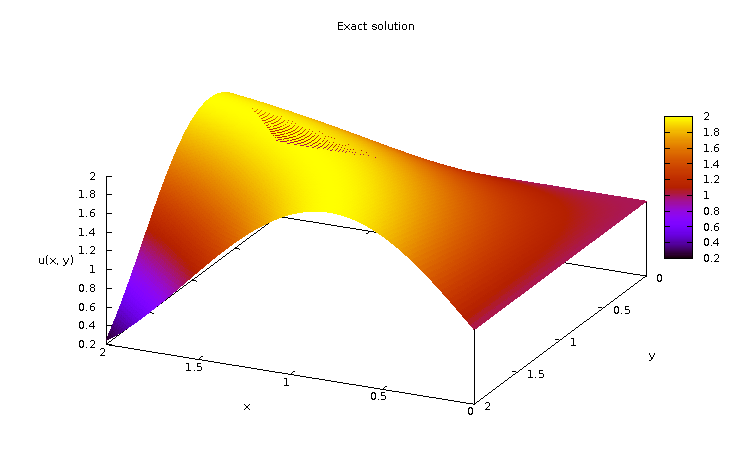
\includegraphics[scale=1.3]{correct_sol.pdf}
  \caption{Точное решение для решётки $100 \times 100$}
  \label{exact:image}
\end{figure}

На рис.~\ref{parallel:image} показан график полученного приближения для решётки
размера $100 \times 100$. Слегка разная расцветка объясняется тем, что в точках
где точное значение функции равно 2, приближенное оказывается иногда немного
больше, и под такие точки пришлось завести отдельный числовой диапазон с
дополнительным цветовым переходом.

\begin{figure}[h]
  \centering
  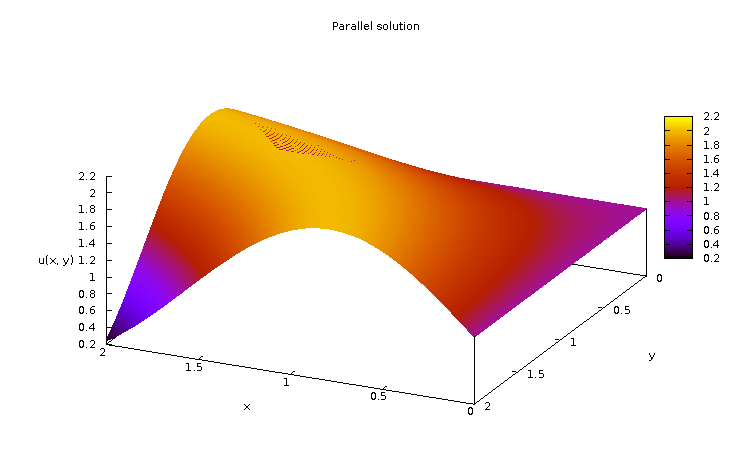
\includegraphics[scale=1.3]{mine_sol.pdf}
  \caption{Приближенное решение для решётки $100 \times 100$}
  \label{parallel:image}
\end{figure}

На рис.~\ref{err:image} приведена абсолютная погрешность приближенного решения
для все той же решётки размера $100 \times 100$. Поскольку строить подобные
графики для решёток больших размерностей нецелесообразно, в табл.~\ref{err:table}
приведена максимальная среди всех точек погрешность для некоторых других размеров
решеток.

\begin{figure}[h]
  \centering
  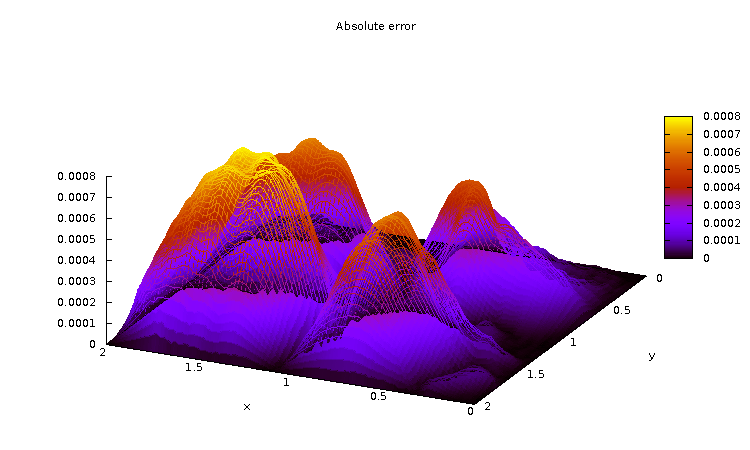
\includegraphics[scale=1.3]{abs_error.pdf}
  \caption{Погрешность приближенного решения для решётки $100 \times 100$}
  \label{err:image}
\end{figure}


\begin{table}[h]
  \centering
  \caption{Максимальная погрешность для разных решёток}
  \label{err:table}
  \begin{tabular}{|l|l|}
    \hline
    \textbf{Размер решетки}    & \textbf{Максимальная погрешность} \\ \hline
    100  & 0.00079142450755                  \\ \hline
    1000                       & 0.00772543579084                  \\ \hline
    2000 & 0.00784839234615                  \\ \hline
  \end{tabular}
\end{table}


\end{document}